\subsection{Loop shaping}
The Bode plots of our open-loop system are given at figure \ref{fig:bode-ol}.
\begin{figure}[H]
    \centering
    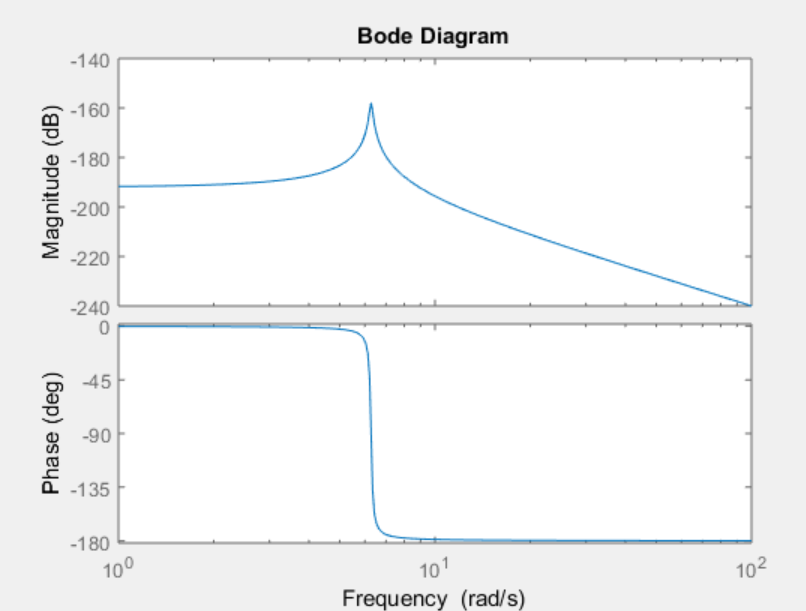
\includegraphics[width=0.8\textwidth]{resources/png/bode-ol.png}
    \caption{Bode plots for 2D system.}
    \label{fig:bode-ol}
\end{figure}
As can be seen, every frequency is well attenuated, the high ones as well as the low ones.\par
At the cross-over frequency, the gain of the system is of about \SI{-215}{\deci\bel}. This is not what we want. We would like low frequencies to have a positive gain, high frequencies to have a negative one and the gain at the crossover frequency to be of \SI{0}{\deci\bel}.\par
Furthermore, we need a big enough phase margin at the crossover frequency to be resistant to the delays we will have in our system. In order to do that, we have decided to use a lead compensator as well as a gain. We will not need a low-pass filter as high frequencies will be well attenuated without it.

% Lead compensator
\subsubsection{Lead compensator}
Let's first start with the desired phase margin. Delays are discussed after, but we want to be able to respond at least to \SI{0.02}{\second} delays, which correspond to the \SI{50}{\hertz} of the actuator's piston \cite{iopscience_delay}.\par
We have decided to have a phase margin of \SI{70}{\degree}. In order to increase the phase margin at the crossover frequency, we have decided to use a lead compensator.\par
Its transfer function is given by : 
$$
G(s) = \dfrac{\frac{s}{w_z} + 1}{\frac{s}{w_p} +1}
$$
We now have to determine the values of the parameters $G_{LC}$, $w_z$ and $w_p$. For a given crossover frequency $\omega_{co}$ and a phase margin $\phi_m$, we can determine the two $w$ in the following way : 
$$
\left\{\begin{array}{l}
    {w_{z}=\tan (\alpha) w_{\mathrm{co}}} \\
    {w_{p}=\frac{w_{\mathrm{co}}}{\tan (\alpha)}}
\end{array}\right.
$$
with $\alpha = \frac{\pi}{4} - \frac{\phi_m}{2}$.\par
For our crossover frequency and our desired value of $\phi_m$, we get that : 
$$
w_z = \num{5.2898} \qquad w_p = \num{170.1385}
$$

% Gain
\subsubsection{Gain}
After that, we need to add a gain to our system in order to increase the amplitude gains for all frequencies and make it so that the amplitude is at \SI{0}{\deci\bel} at the crossover frequency. That is done by using a constant gain of \num{1.5178e9}. This does not affect the phase but increases the amplitudes of about \SI{183.6}{\deci\bel}, which positions our Bode plot to where we wanted it to be.

% Trade-offs
\subsubsection{Trade-offs}
The Bode and Nyquist plots of the controlled system are given at figures \ref{fig:bode-control} and \ref{fig:nyquist-control}. As can be seen, the desired results are obtained, and we have a phase margin of \SI{70}{\degree} on the Nyquist plot.
\begin{figure}[H]
    \centering
    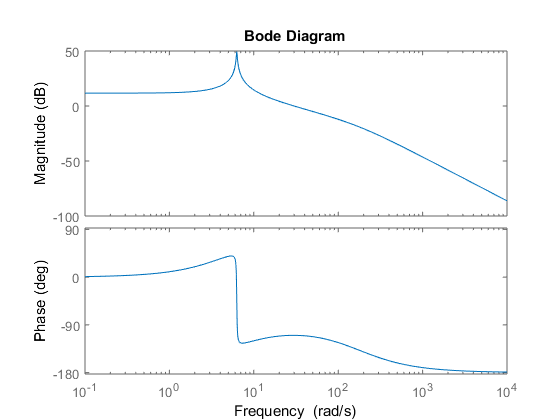
\includegraphics[width=0.8\textwidth]{resources/png/bode-control.png}
    \caption{Bode plots of the controlled system}
    \label{fig:bode-control}
\end{figure}
\begin{figure}[H]
    \centering
    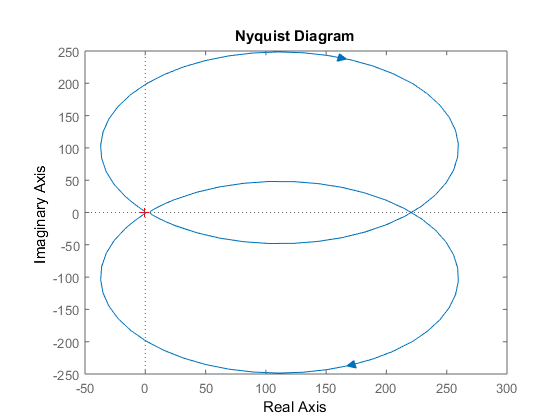
\includegraphics[width=0.8\textwidth]{resources/png/nyquist-control.png}
    \caption{Nyquist plot of the controlled system}
    \label{fig:nyquist-control}
\end{figure}
Concerning the impacts on the output signal and control input signal, they are in an acceptable range of values with the parameters we have chosen, as can be seen in figures \ref{fig:controllable-input} and \ref{fig:output}.
\begin{figure}[H]
    \centering
    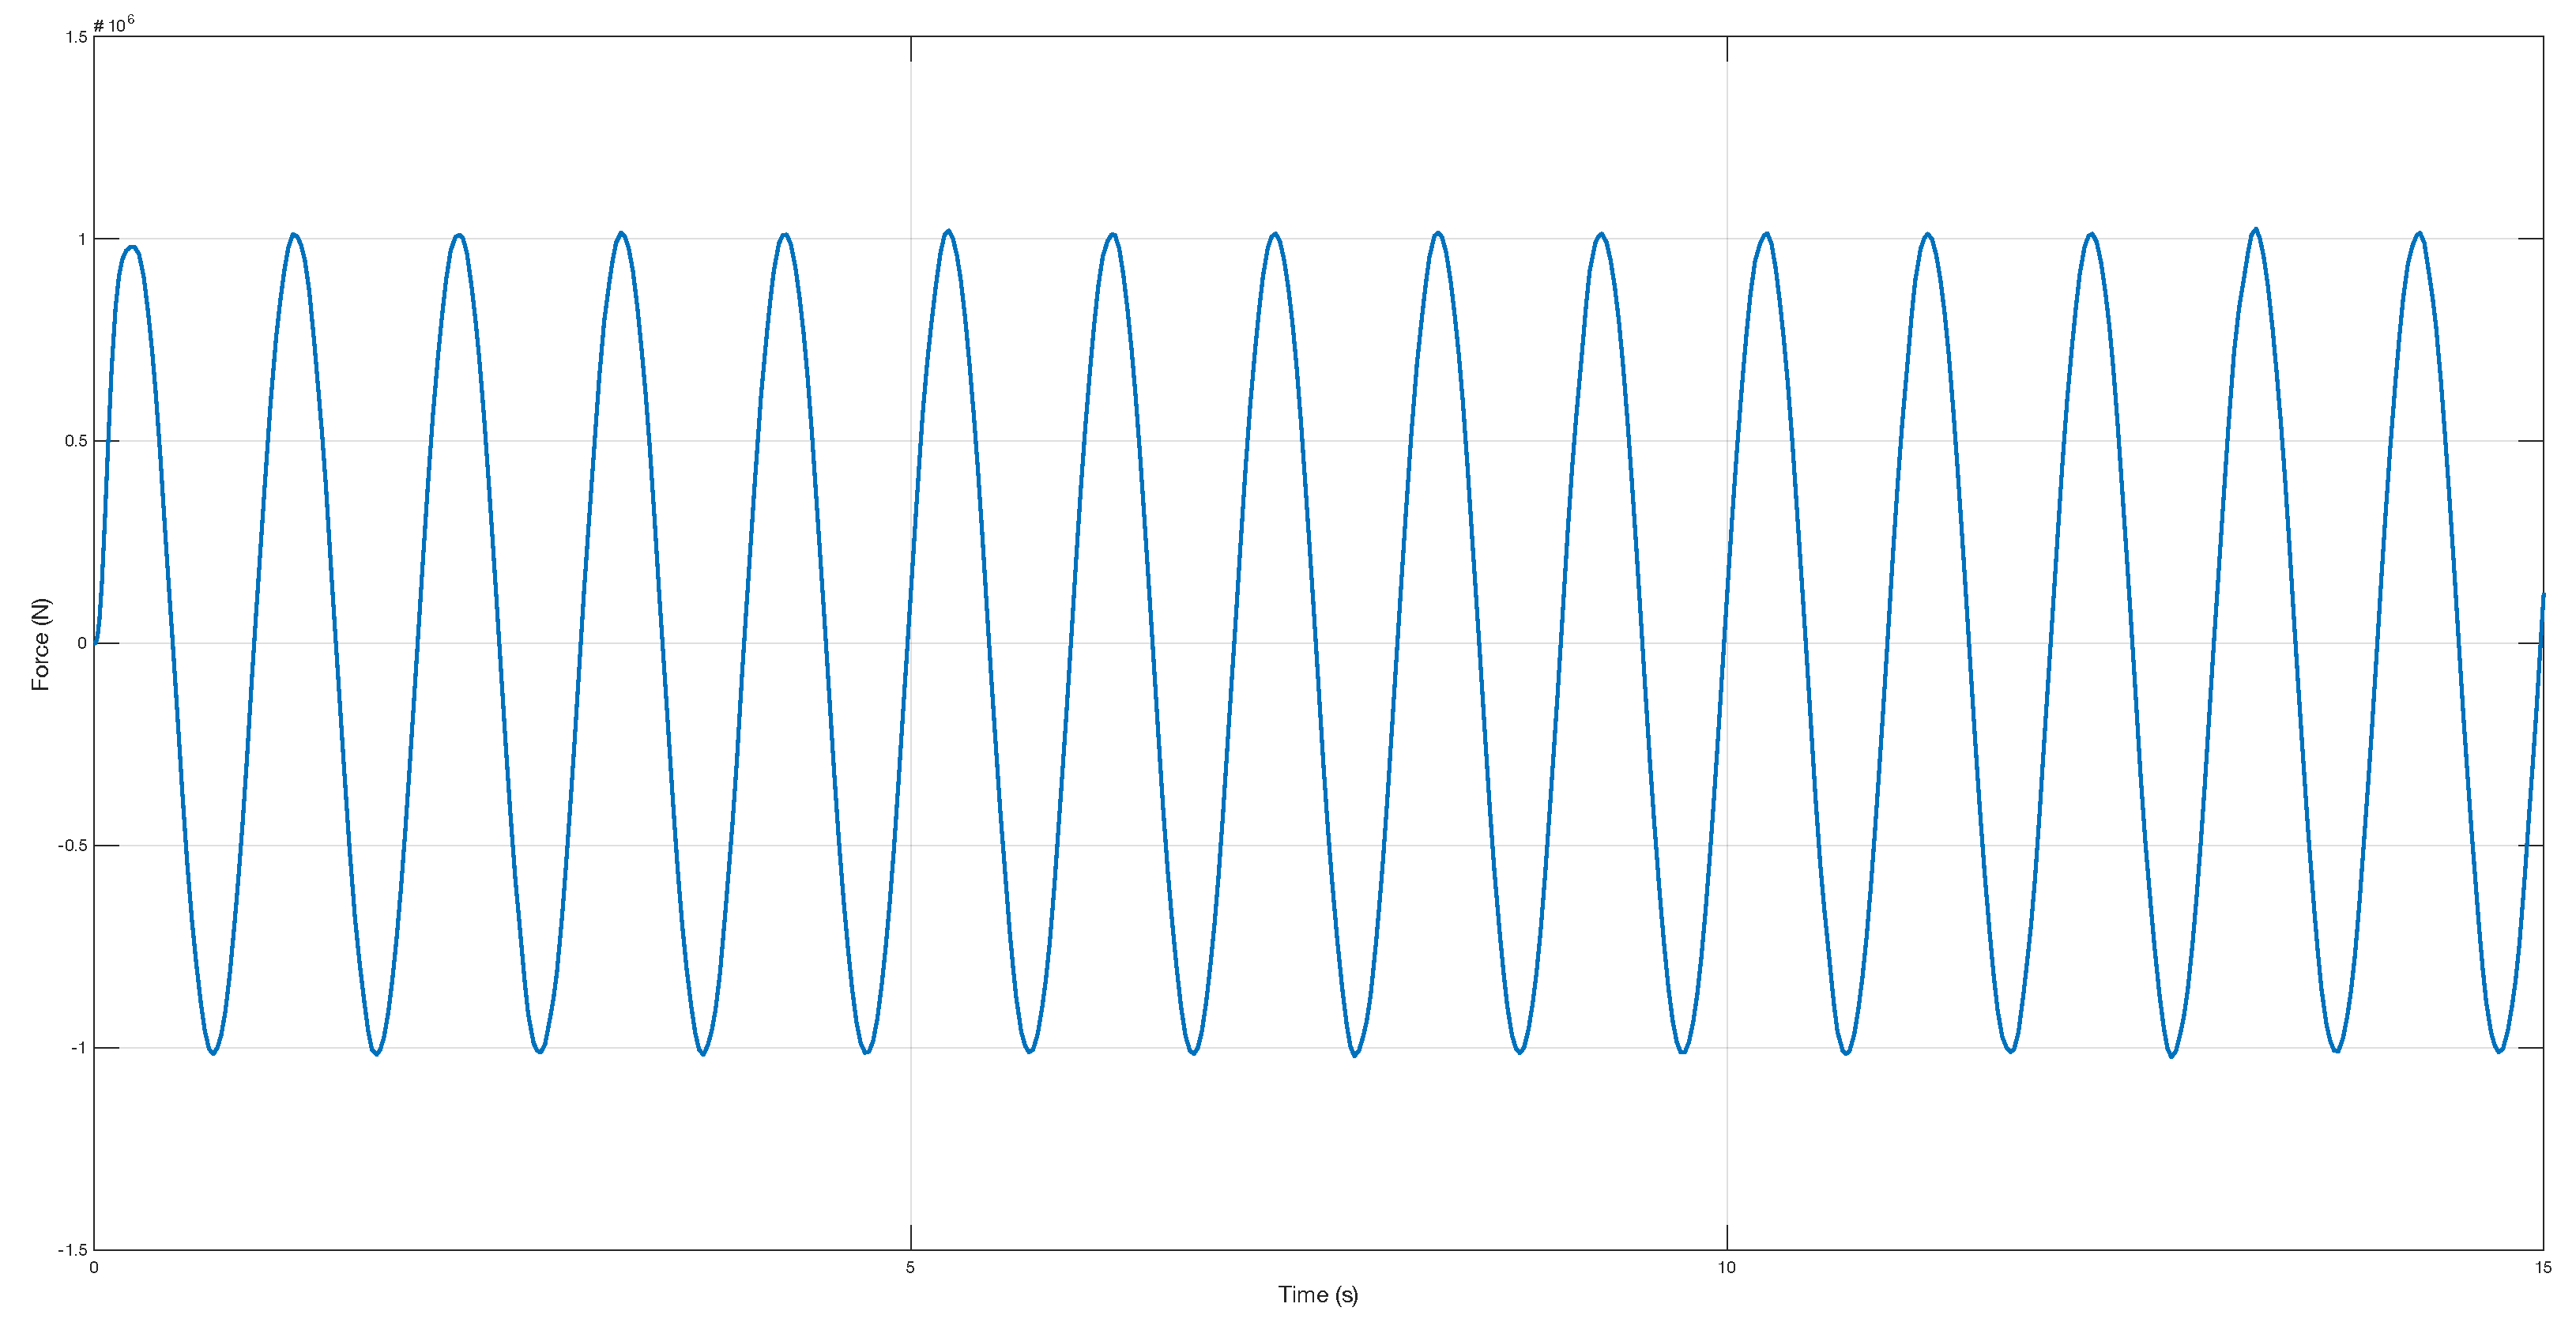
\includegraphics[width=0.8\textwidth]{resources/pdf/controllable-input.pdf}
    \caption{Plot of the controllable input of the controlled system}
    \label{fig:controllable-input}
\end{figure}
\begin{figure}[H]
    \centering
    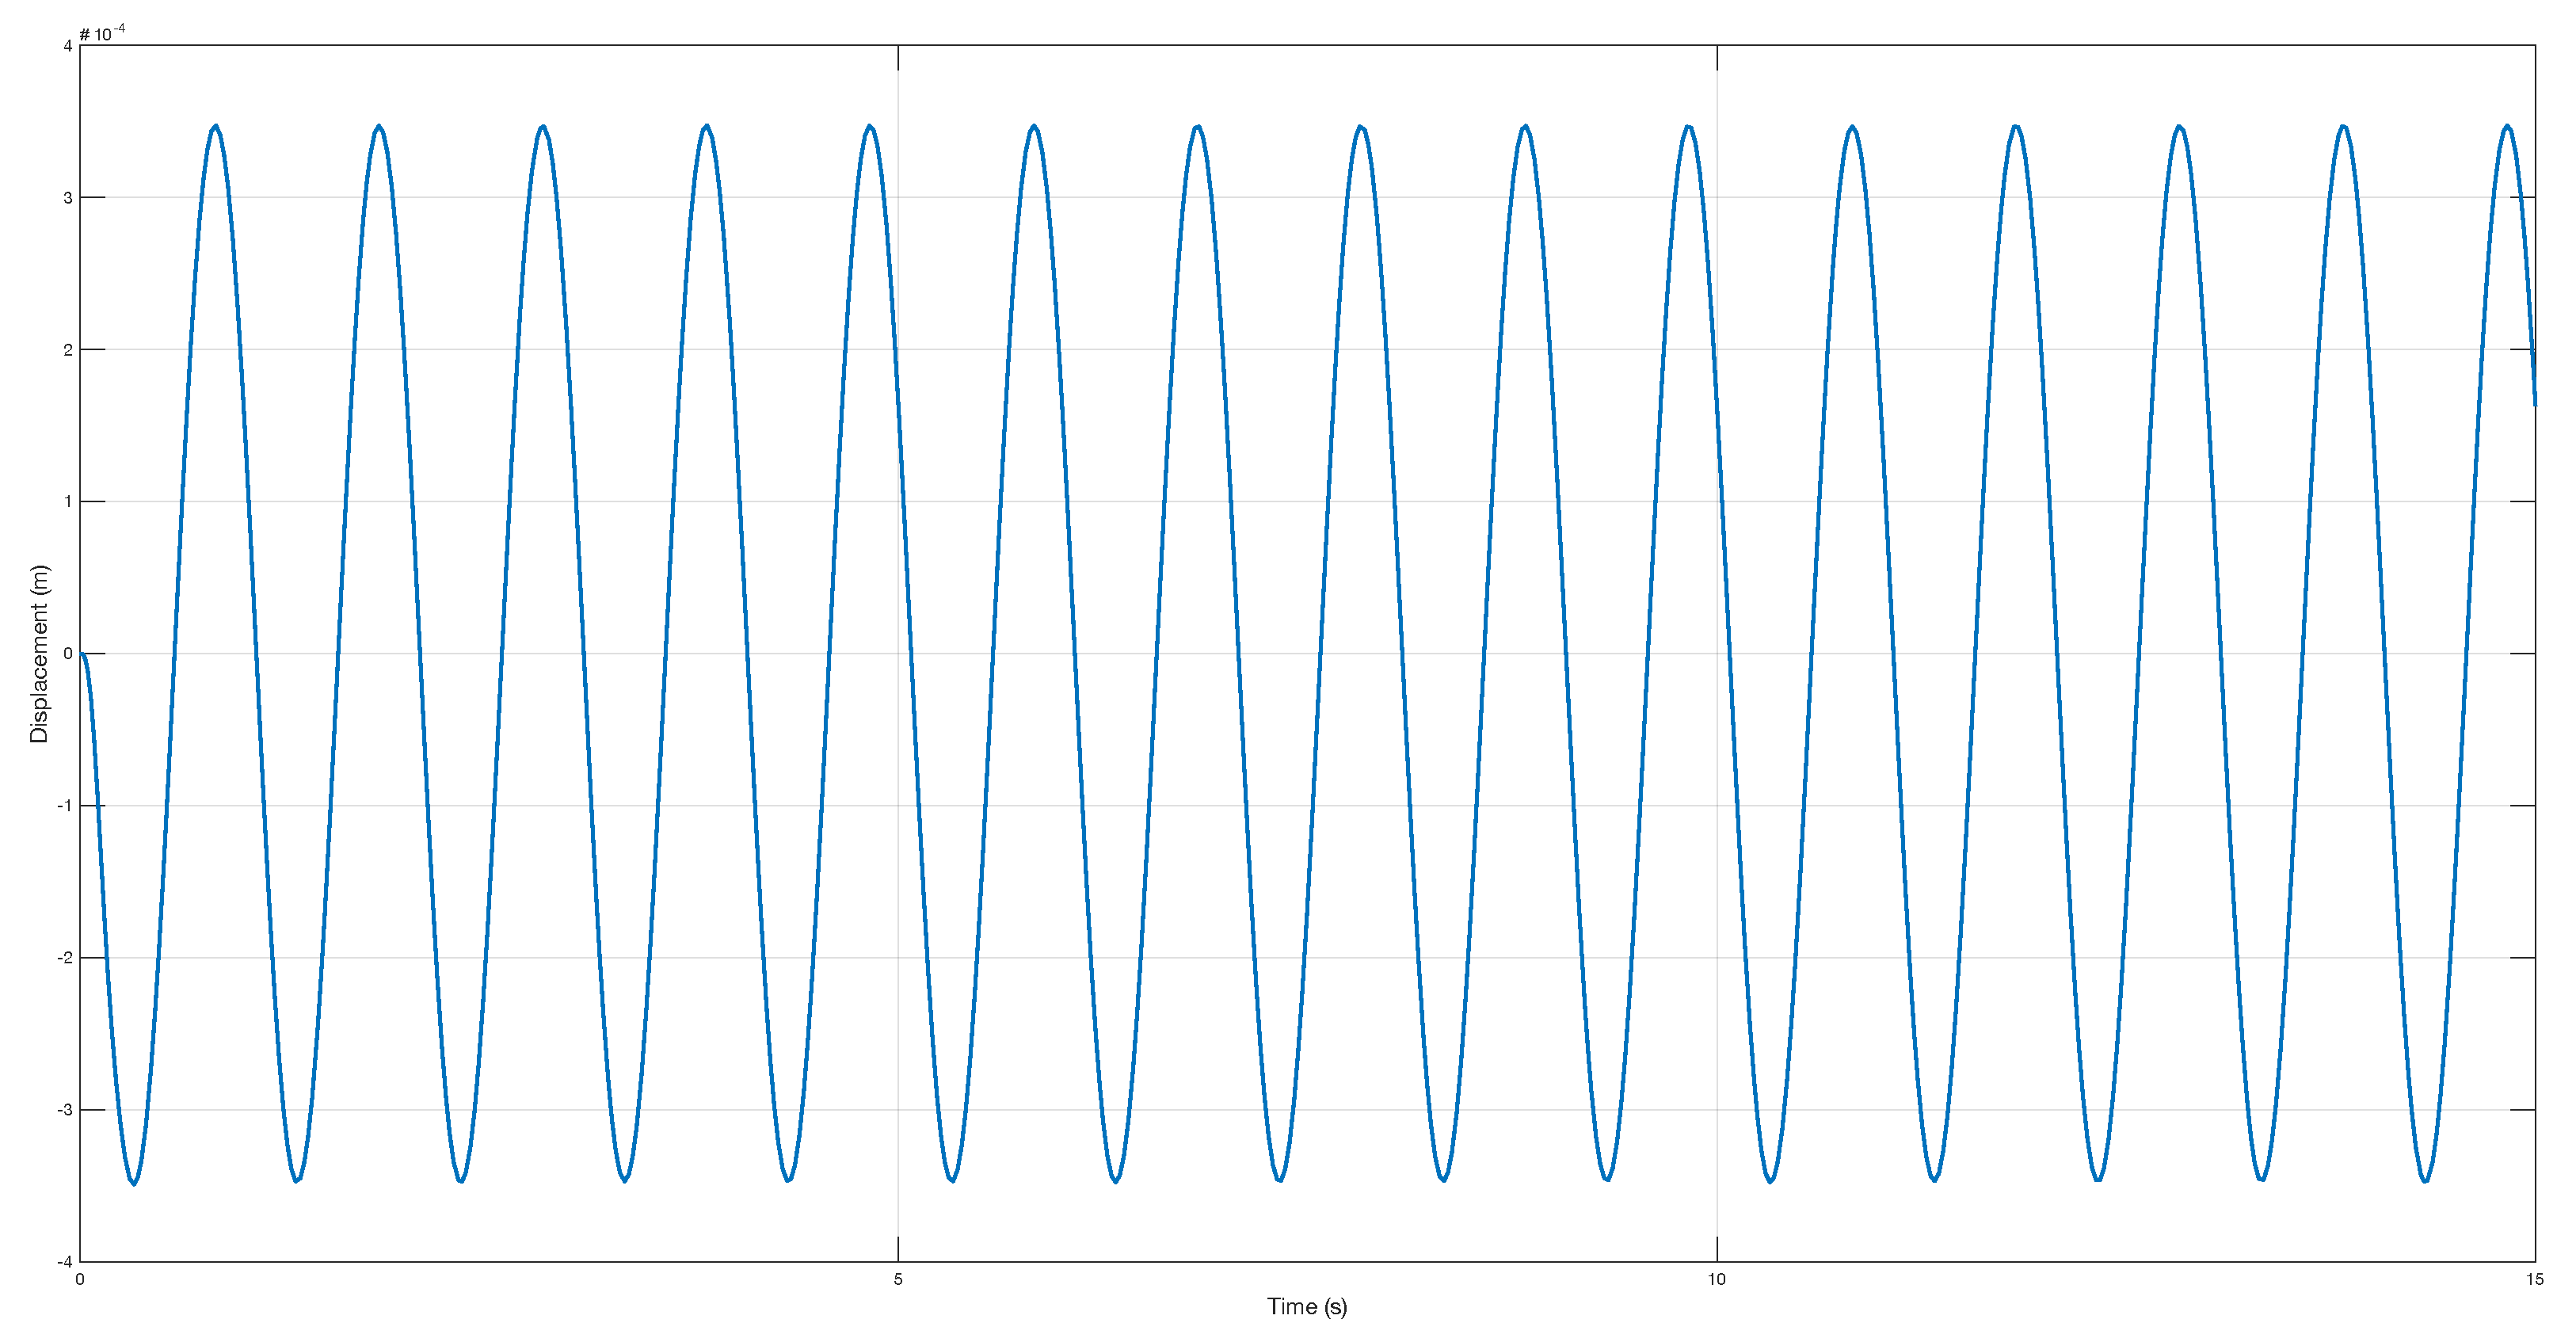
\includegraphics[width=0.8\textwidth]{resources/pdf/output.pdf}
    \caption{Plot of the output of the controlled system}
    \label{fig:output}
\end{figure}
